\documentclass[12pt]{article}
\usepackage[table,xcdraw]{xcolor}
\usepackage{multirow}
\usepackage{pdflscape}
\usepackage{amsmath}
\usepackage{amsfonts}
\usepackage{float}
\usepackage{fancyhdr}
\usepackage{graphicx}
\usepackage{hyperref}
\usepackage{indentfirst}
\usepackage{url}
\usepackage{subfig}
\usepackage[top=.75in, left=.75in, right=.75in, bottom=1in]{geometry}
\usepackage{gensymb}
\hypersetup{
    colorlinks=true,
    linkcolor=blue,
    filecolor=magenta,      
    urlcolor=cyan,
    pdftitle={Overleaf Example},
    pdfpagemode=FullScreen,
    }
%\usepackage[utf8]{vietnam}

% For algorithm
\usepackage{algorithm}
\usepackage{algpseudocode}

% ============ CODE ============
\usepackage{listings} 
\usepackage{xcolor}
\definecolor{codegreen}{rgb}{0,0.6,0}
\definecolor{codegray}{rgb}{0.5,0.5,0.5}
\definecolor{codepurple}{rgb}{0.58,0,0.82}
\definecolor{backcolour}{rgb}{0.95,0.95,0.92}

% Styling for the code.
\lstdefinestyle{mystyle}{
    backgroundcolor=\color{backcolour},   
    commentstyle=\color{codegreen},
    keywordstyle=\color{magenta},
    numberstyle=\tiny\color{codegray},
    stringstyle=\color{codepurple},
    basicstyle=\ttfamily\footnotesize,
    breakatwhitespace=false,         
    breaklines=true,                 
    captionpos=b,                    
    keepspaces=true,                 
    numbers=left,                    
    numbersep=5pt,                  
    showspaces=false,                
    showstringspaces=false,
    showtabs=false,                  
    tabsize=2
}
\lstset{style=mystyle}

% Disable indentation on new paragraphs
\setlength{\parindent}{0pt}

% Optional: graphic path
% \graphicspath{PATH_TO_GRAPHIC_FOLDER}

% To use Times font family, uncomment this row
% \usepackage{mathptmx}

% To use roman section / subsection, uncomment these rows
% \renewcommand{\thesection}{\Roman{section}}
% \renewcommand{\thesubsection}{\thesection.\Roman{subsection}}

% Define course name, report name and report title.
\newcommand{\coursename}{Data Structures and Algorithms}
\newcommand{\reportname}{MOOC Report}
\newcommand{\reporttitle}{Report}
\newcommand{\studentname}{Nguyen Le Ho Anh Khoa - 23127211}
\newcommand{\teachername}{Bui Duy Dang \\ Truong Tan Khoa \\ Nguyen Thanh Tinh}

% ============ HEADER AND FOOTER ============
% Header length
\setlength{\headheight}{29.43912pt}

% Footer page number would be on the lower-right corner
\pagestyle{fancy}
\fancyfoot{}
\fancyfoot[R]{Page \thepage}

\lhead{\reportname}
\rhead{VNUHCM-US\\
\coursename
}
% Remove the \leftfooter command from the footer definition
\lfoot{}

%Footer page number for landscape
\fancypagestyle{lscape}{
\fancyhf{}
\fancyfoot[R]{Page \thepage}
\renewcommand{\headrulewidth}{0pt} 
  \renewcommand{\footrulewidth}{0pt}
}



% ============ DOCUMENT ============
\begin{document}
\begin{titlepage}
\newcommand{\HRule}{\rule{\linewidth}{0.5mm}}
\centering

\textsc{\LARGE vietnam national university of \\ho chi minh city}\\[0.8cm]
\textsc{\Large university of science}\\[0.4cm]
\textsc{\large faculty of information technology}\\[0.4cm]

\HRule \\[0.4cm]
{ 
\Large{\bfseries{\reporttitle}}\\[0.4cm]
\huge{\bfseries{\reportname}}
}\\[0.4cm]
\HRule \\[0.4cm]

\textbf{\large Course name: \coursename}\\[0.4cm]
\textbf{\large CSC10004\textunderscore23CLC09} \\ [0.7cm]
\begin{minipage}[t]{0.4\textwidth}
\begin{flushleft} \large
\emph{Students:}\\
\studentname
\end{flushleft}
\end{minipage}
~
\begin{minipage}[t]{0.4\textwidth}
\begin{flushright} \large
\emph{Teacher:} \\
\teachername
\end{flushright}
\end{minipage}\\[0.7cm]

{\large \today}\\[1cm]


\includegraphics[scale=1.1]{img/hcmus-logo.png}\\[0cm] 

\vfill
\end{titlepage}
	
\tableofcontents
\pagebreak
\section{Student Information}
Class: 23CLC09 \\
Student ID: 23127211 \\
Full name: Nguyen Le Ho Anh Khoa
\section{Summary of the courses}
\subsection{Algorithm Toolbox |
	University of California San Diego | Cousera}

\begin{figure}[H]
	\centering
	
\includegraphics[width=0.7\linewidth]{img/Cert01.png}
	\caption{Algorithm Toolbox Certificate on Cousera}
	\label{fig:algorithmtoolbox}
\end{figure}

\begin{figure}[H]
	\centering
	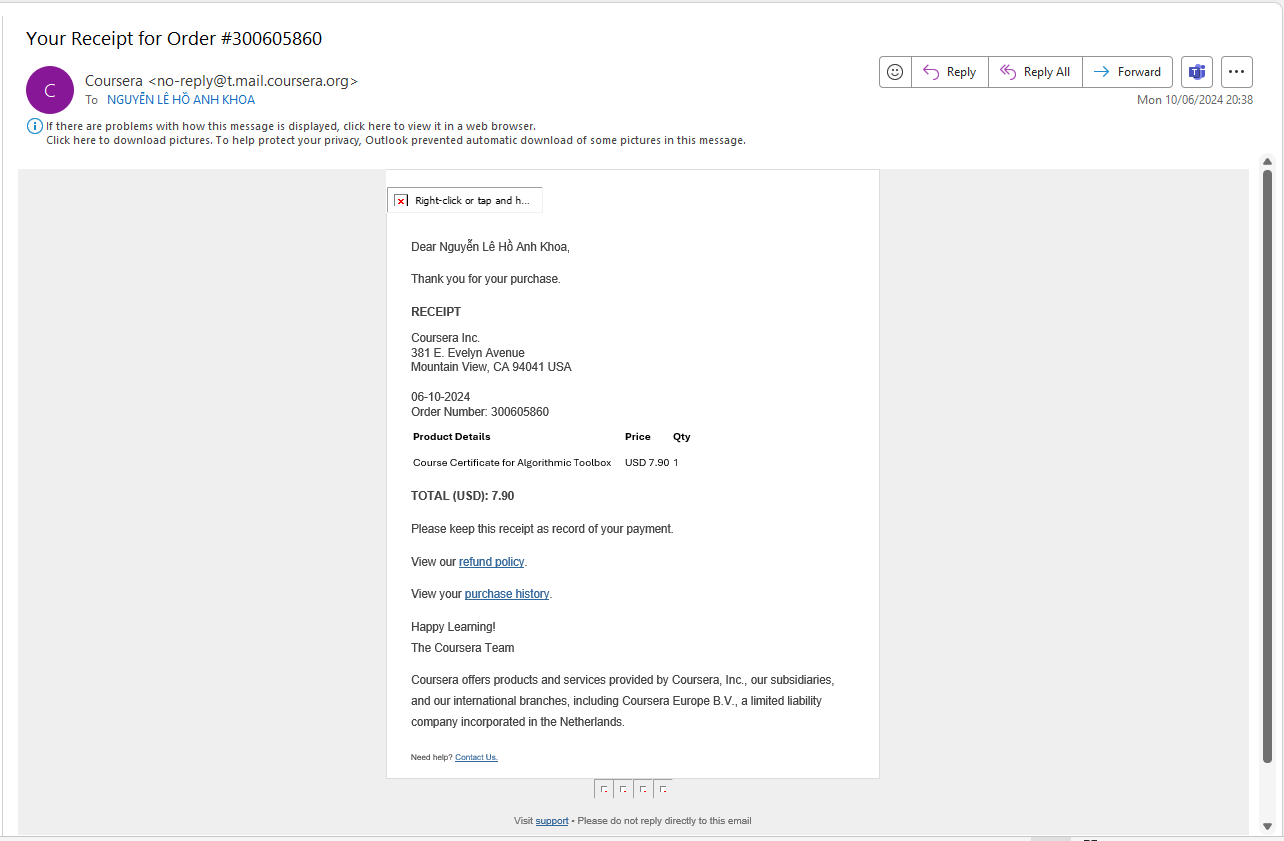
\includegraphics[width=0.7\linewidth]{img/Capture01.PNG}
	\caption{Algorithm Toolbox Course start on Jun 10 2024}
	\label{fig:algorithmtoolbox}
\end{figure}

\begin{figure}[H]
	\centering
	
\includegraphics[width=0.7\linewidth]{img/Capture02.PNG}
	\caption{Algorithm Toolbox Course completed on August 7 2024}
	\label{fig:algorithmtoolbox}
\end{figure}

\begin{figure}[H]
	\centering
	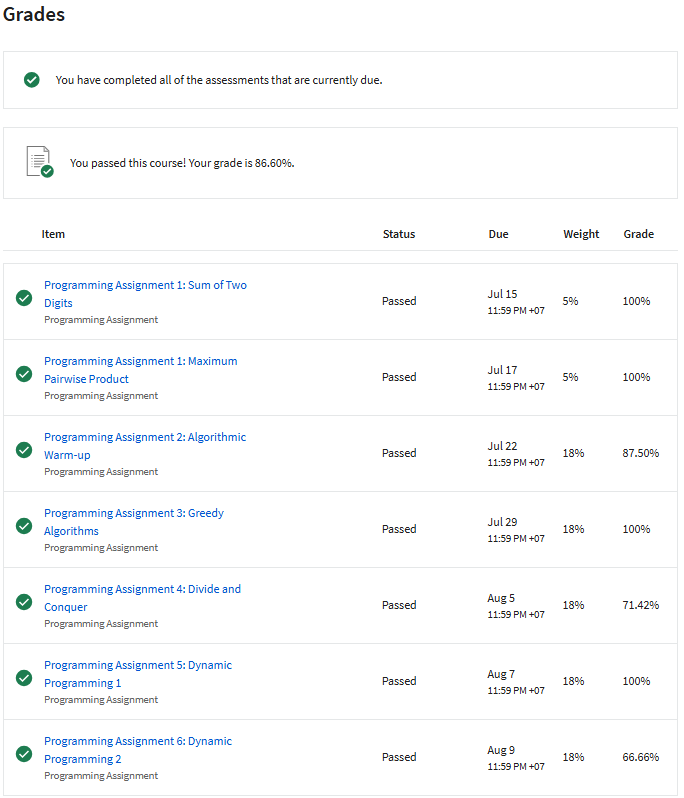
\includegraphics[width=0.7\linewidth]{img/Capture06.PNG}
	\caption{Graded of Algorithm Toolbox Course}
	\label{fig:algorithmtoolbox}
\end{figure}

\subsubsection{Course Introduction}
\begin{itemize}
	\item \textbf{Course Name:} Algorithm Toolbox
	\item \textbf{Institution:} University of California San Diego
	\item \textbf{Platform:} Cousera
	\item \textbf{Level: } Intermediate
	\item \textbf{Commitment:} 5 weeks, 4-8 hours per week
	\item \textbf{Instructor:} Pavel Pevzner, Michael Levin
	\item \textbf{Course Link:} \href{https://www.coursera.org/learn/algorithmic-toolbox}{Algorithm Toolbox}
\end{itemize}

\subsubsection{Course Content}
This is Course 1 of 6 in the \href{https://www.coursera.org/specializations/data-structures-algorithms}{Data Structures and Algorithms Specialization} \\

I am taking this course to supplement my university course on Data Structures and Algorithms. This online course provides additional practice and deeper insights into algorithmic techniques, which will help me better understand and apply the concepts taught in my university course.\\

The course content is divided into six modules:
\begin{itemize}
	\item \textbf{Module 1: Introduction: Asymptotic Analysis and Getting Started with Programming Challenges.} In this module, students are introduced to algorithmic thinking and asymptotic analysis. Basic programming challenges are provided to help students get started.
	\item \textbf{Module 2: Algorithmic Warm-up: Fibonacci Numbers and the Greatest Common Divisor.} This module covers efficient computation of Fibonacci numbers and algorithms for finding the greatest common divisor (GCD).
	\item \textbf{Module 3: Greedy Algorithms: Minimum Spanning Trees, Clustering, Huffman Codes.} This module I learn about greedy algorithms and their applications in minimum spanning trees, clustering, and Huffman coding for data compression.
	\item \textbf{Module 4: Divide and Conquer: Sorting and Searching, QuickSort, Binary Search Trees.} This module introduces the divide and conquer strategy, sorting algorithms like QuickSort, and binary search trees for efficient searching.
	\item \textbf{Module 5: Dynamic Programming: Edit Distance, Knapsack.} I am introduced to dynamic programming, solving the edit distance problem, and the knapsack problem and its variations.
	\item \textbf{Module 6: Dynamic Programming 2: Advanced Topics, Longest Common Subsequence, Overlapping Subproblems.} This module covers advanced topics in dynamic programming, the longest common subsequence problem, and handling overlapping subproblems.
\end{itemize}

\subsection{Data Structures |
	University of California San Diego | Cousera}
\begin{figure}[H]
	\centering
	
\includegraphics[width=0.7\linewidth]{img/Cert02.png}
	\caption{Data Structures Certificate on Cousera}
	\label{fig:datastructures}
\end{figure}

\begin{figure}[H]
	\centering
	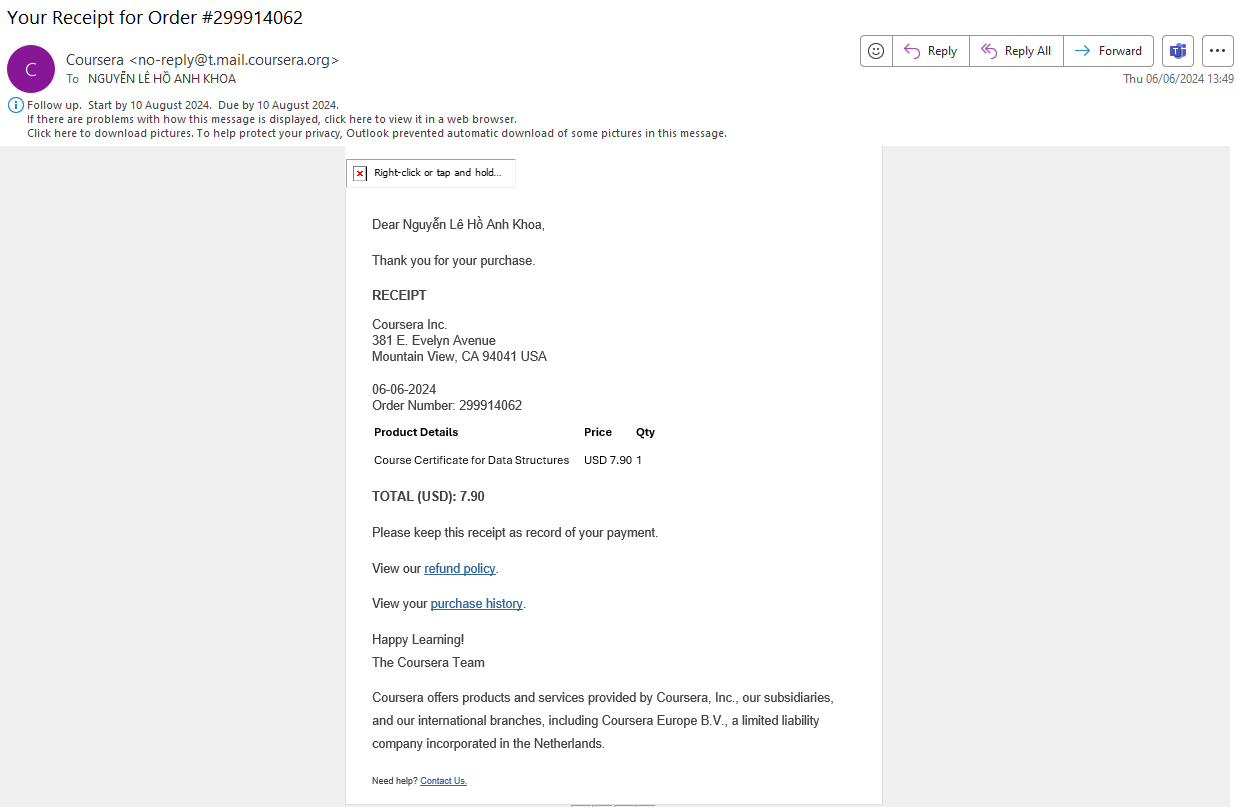
\includegraphics[width=0.7\linewidth]{img/Capture03.PNG}
	\caption{Data Structures Course start on Jun 6 2024}
	\label{fig:algorithmtoolbox}
\end{figure}

\begin{figure}[H]
	\centering
	
\includegraphics[width=0.7\linewidth]{img/Capture04.PNG}
	\caption{Data Structures Course completed on August 5 2024}
	\label{fig:algorithmtoolbox}
\end{figure}

\begin{figure}[H]
	\centering
	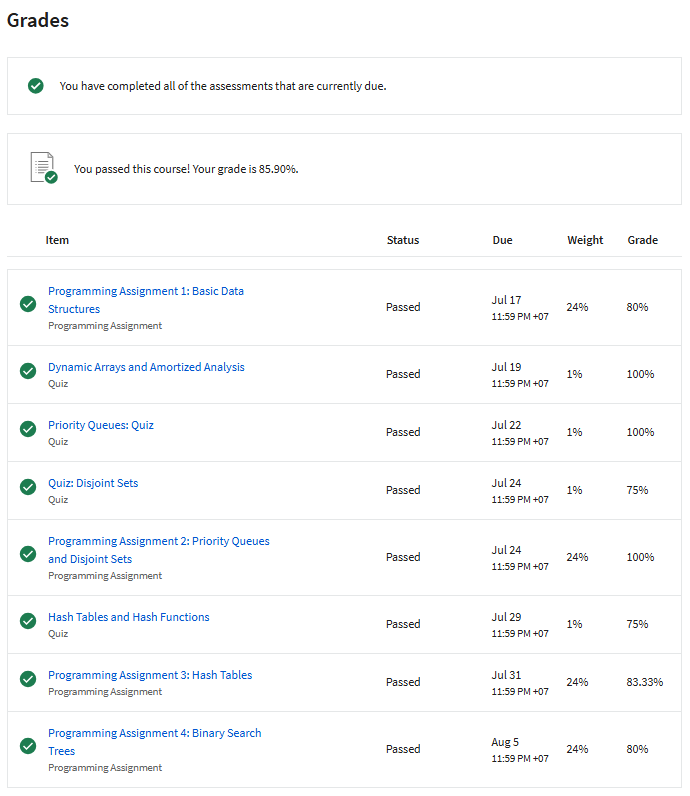
\includegraphics[width=0.65\linewidth]{img/Capture07.PNG}
	\caption{Graded of Data Structures Course}
	\label{fig:algorithmtoolbox}
\end{figure}

\subsubsection{Course Introduction}
\begin{itemize}
	\item \textbf{Course Name:} Data Structures
	\item \textbf{Institution:} University of California San Diego
	\item \textbf{Platform:} Cousera
	\item \textbf{Level: } Intermediate
	\item \textbf{Commitment:} 5 weeks, 4-8 hours per week
	\item \textbf{Instructor:} Pavel Pevzner, Michael Levin
	\item \textbf{Course Link:} \href{https://www.coursera.org/learn/data-structures}{Data Structures}
\end{itemize}
\subsubsection{Course Content}
This is Course 2 of 6 in the \href{https://www.coursera.org/specializations/data-structures-algorithms}{Data Structures and Algorithms Specialization}. \\

This is an opportunity for me to consolidate my knowledge at school. By engaging in this process, I can reinforce the concepts and skills I have learned, ensuring a deeper understanding and retention of the material. Additionally, this consolidation will help me identify any gaps in my knowledge, allowing me to address them proactively. Ultimately, this effort will contribute to my overall academic success and prepare me for future challenges. \\

The course content is divided into six modules:
\begin{itemize}
	\item \textbf{Module 1: Basic Data Structures: Arrays, Linked Lists, Stacks, Queues.} In this module, I am introduced to basic data structures including arrays, linked lists, stacks, and queues.
	\item \textbf{Module 2: Trees: Binary Search Trees, AVL Trees, Splay Trees.} This module covers binary search trees and their properties, as well as balanced trees like AVL and Splay trees.
	\item \textbf{Module 3: Hash Tables: Hash Functions, Collisions, Rabin-Karp Algorithm.} Students learn about hash tables and hash functions, handling collisions, and the Rabin-Karp algorithm.
	\item \textbf{Module 4: Priority Queues: Heaps, Heap Sort, Balanced Binary Heaps.} This module introduces priority queues and heaps, including heap sort and balanced binary heaps.
	\item \textbf{Module 5: Hash Tables 2: Open Addressing, Cryptographic Hashing.} This module covers open addressing in hash tables and cryptographic hashing techniques.
	\item \textbf{Module 6: Binary Search Trees: Splay Trees, AVL Trees, Deletion, Randomized BSTs.} This module delves into advanced topics in binary search trees, including deletion operations and randomized binary search trees.
\end{itemize}


\subsection{HTML, CSS, JavaScript, React - Online Certification Course | Udemy}
\begin{figure}[H]
	\centering
	
\includegraphics[width=0.7\linewidth]{img/Cert03.png}
	\caption{HTML, CSS, JavaScript, React Certificate on Udemy completed on August 8 2024}
	\label{fig:htmlcssjsreact}
\end{figure}

\begin{figure}[H]
	\centering
	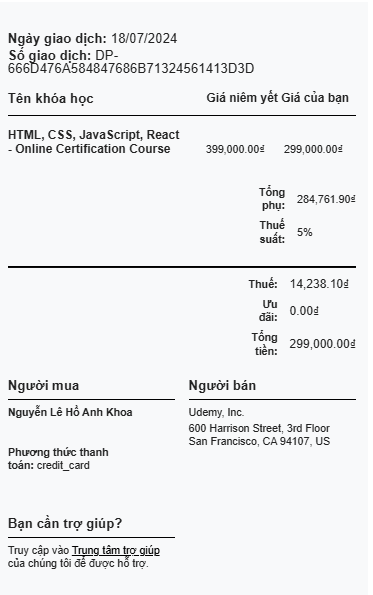
\includegraphics[width=0.7\linewidth]{img/Capture05.PNG}
	\caption{HTML, CSS, JavaScript, React - Online Certification Course start on July 18 2024}
	\label{fig:algorithmtoolbox}
\end{figure}
\subsubsection{Course Introduction}
\begin{itemize}
	\item \textbf{Course Name:} HTML, CSS, JavaScript, React - Online Certification Course
	\item \textbf{Platform:} Udemy
	\item \textbf{Level: } Beginner
	\item \textbf{Commitment:} 4 weeks, 4-6 hours per week
	\item \textbf{Instructor:} YouAccel Training, Blue Digital Media
	\item \textbf{Course Link:} \href{https://www.udemy.com/course/html-css-javascript-react-online-certification-course}{HTML, CSS, JavaScript, React - Online Certification Course}
\end{itemize}
\subsubsection{Course Content}
This course is designed to provide a comprehensive introduction to web development, covering HTML, CSS, JavaScript, and React. By the end of the course, I will have a solid foundation in front-end web development and be able to create interactive and responsive web applications.\\

Udemy is a popular online learning platform that offers a wide range of courses on various topics. The HTML, CSS, JavaScript, React course is designed for beginners who want to learn web development from scratch. The course covers the basics of HTML, CSS, and JavaScript, as well as more advanced topics like React.\\

Udemy don't have system graded like Cousera, so I captured some exercises I did.\\

The course content is divided into four main contents:
\begin{itemize}
	\item \textbf{Content 1: HTML.} In this content, I learn the basics of HTML, including tags, attributes, and elements. I also learn how to create a simple sales website using HTML.
	      \begin{figure}[H]
		      \centering
		      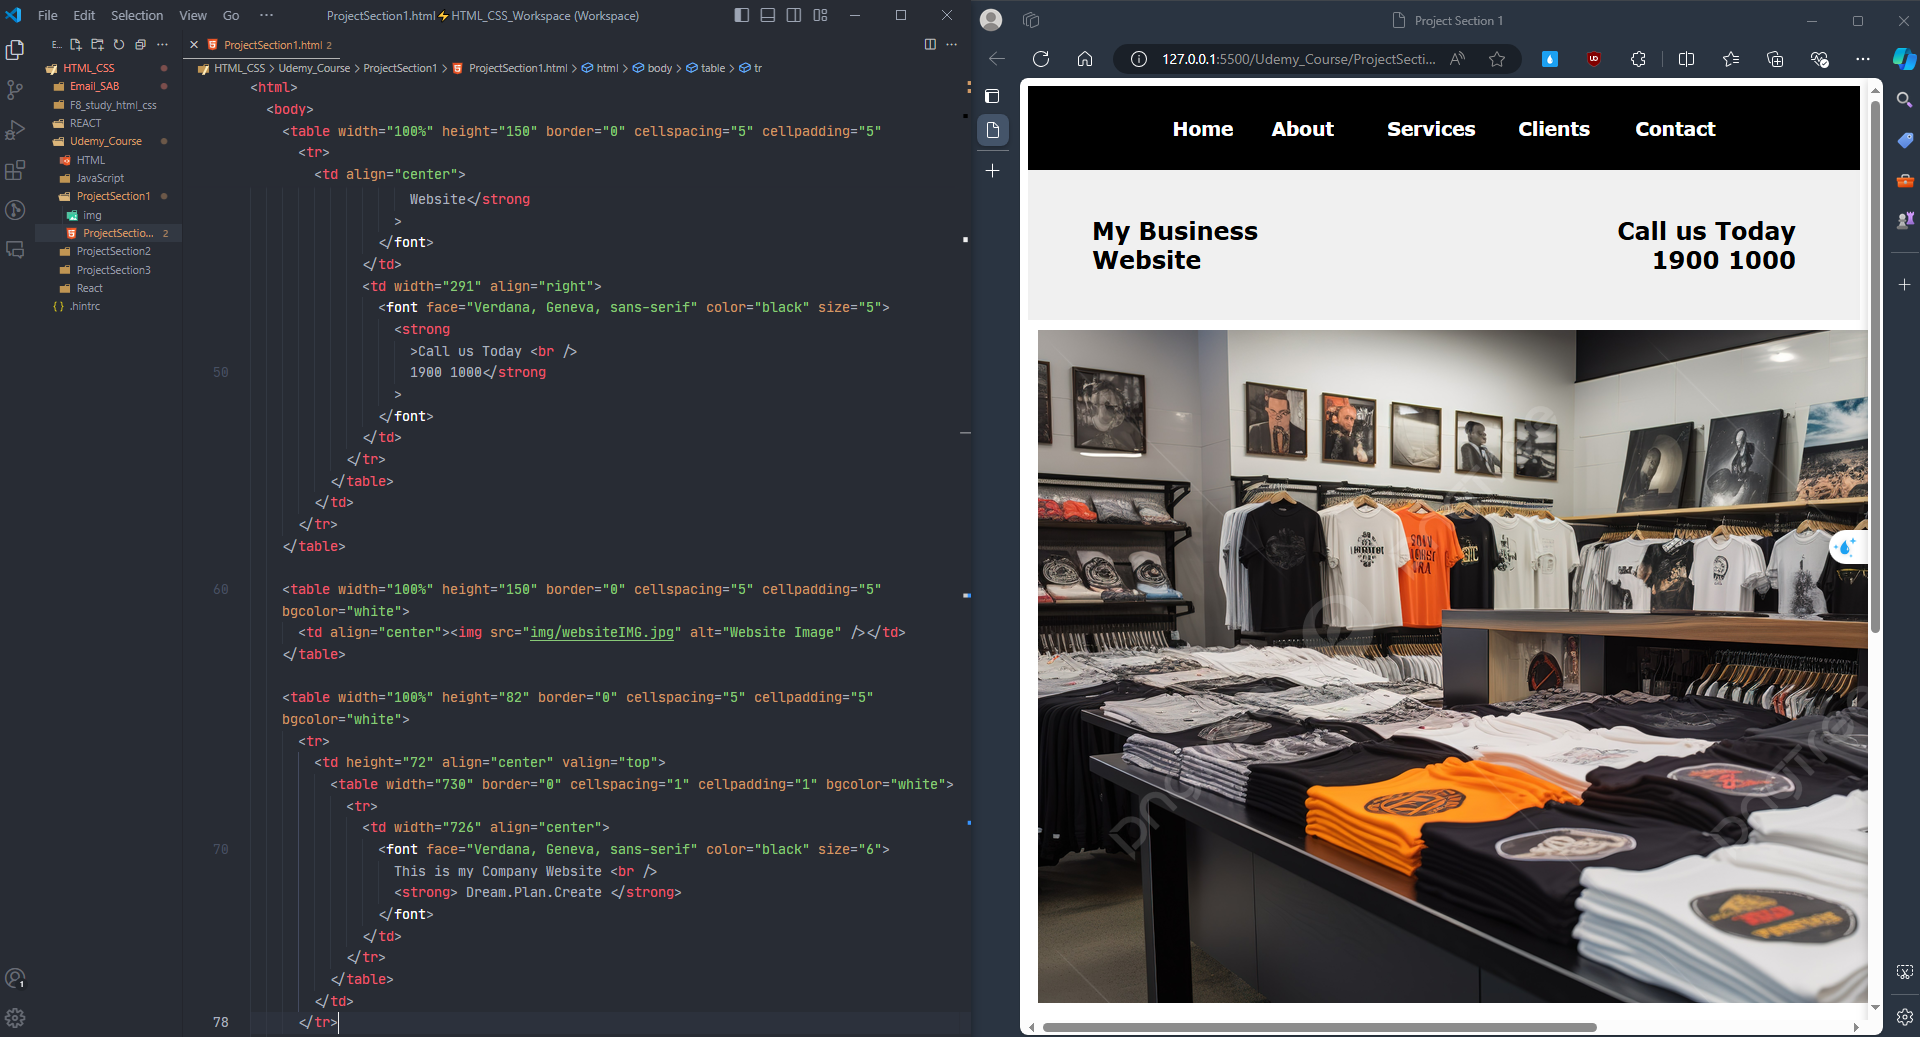
\includegraphics[width=1\linewidth]{img/Capture08.PNG}
		      \caption{A homepage of sales website by HTML}
	      \end{figure}
	\item \textbf{Content 2: CSS.} This content covers CSS fundamentals, including selectors, properties, and values. I learn how to style the sales website created in the previous module using CSS.
	      \begin{figure}[H]
		      \centering
		      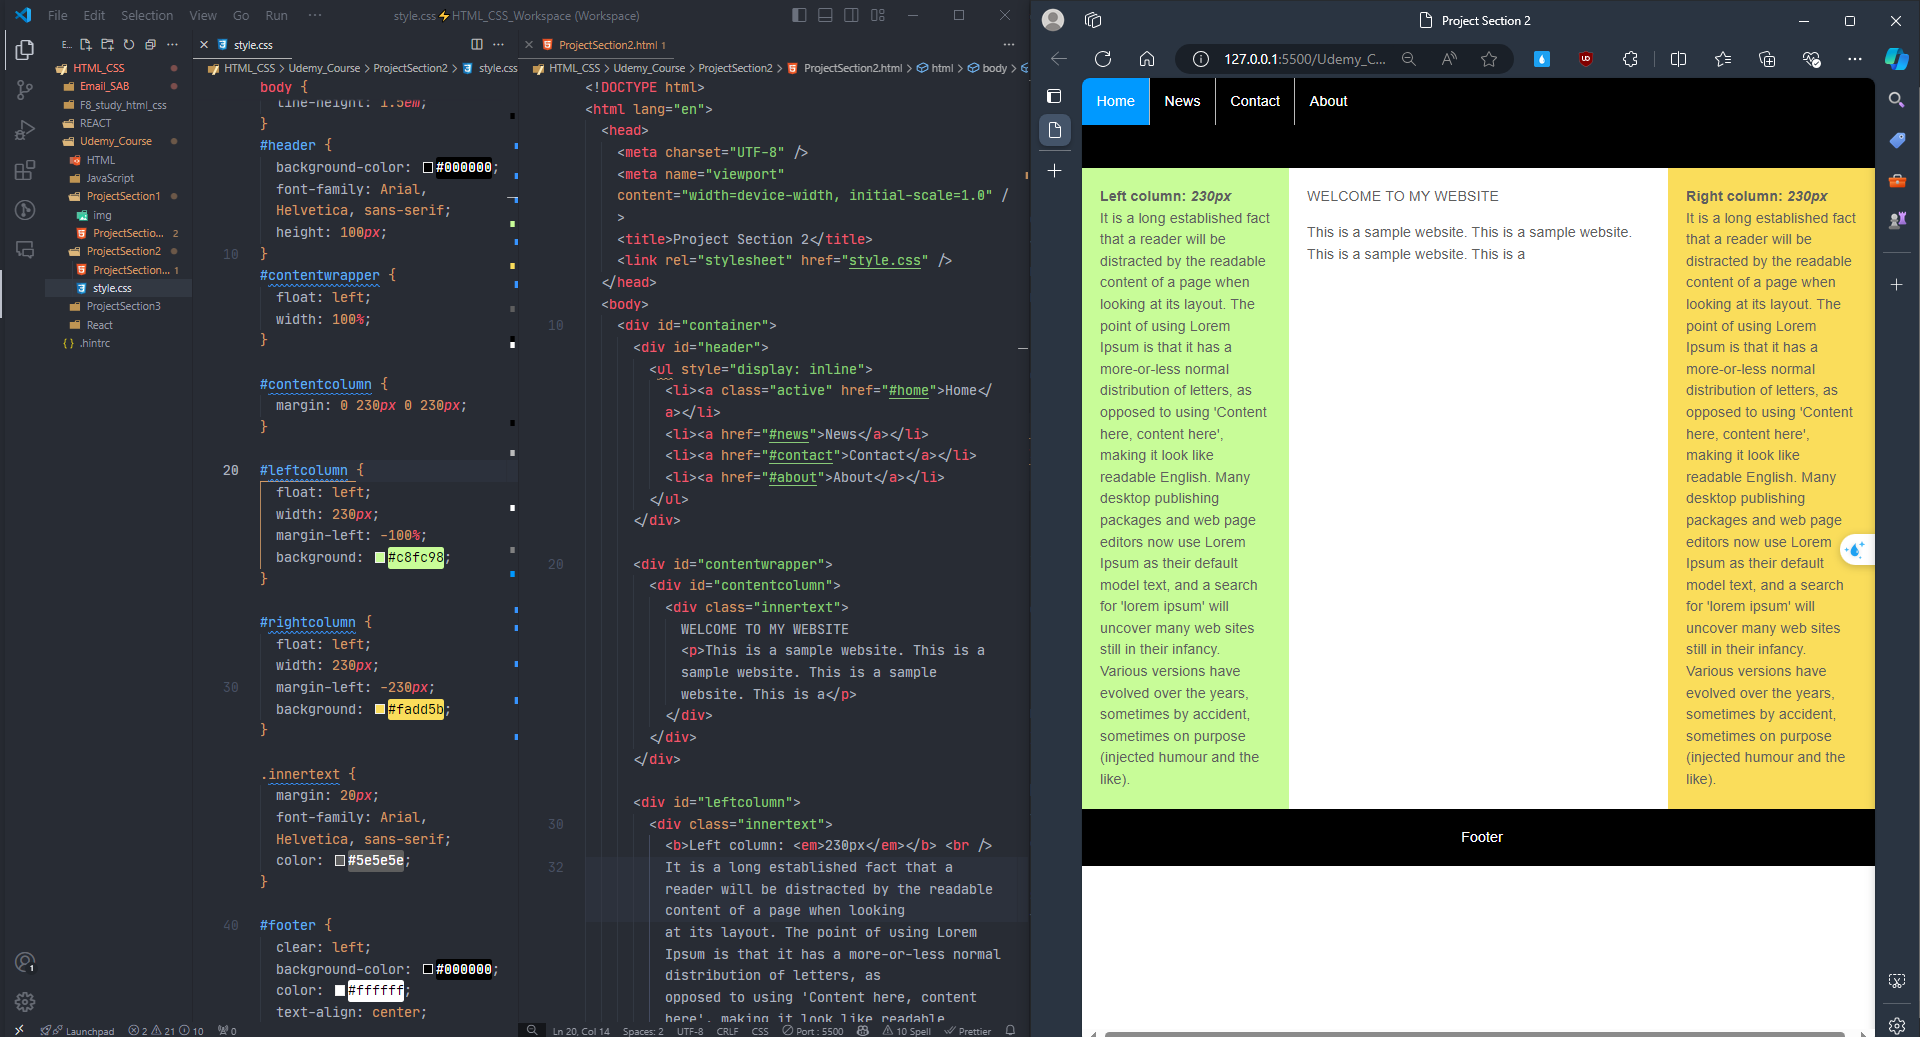
\includegraphics[width=0.9\linewidth]{img/Capture09.PNG}
		      \caption{A demo homepage of a blog website by HTML and CSS}
	      \end{figure}
	\item \textbf{Content 3: JavaScript.} This content covers JavaScript fundamentals, including variables, data types, functions, and control structures.
	      \begin{figure}[H]
		      \centering
		      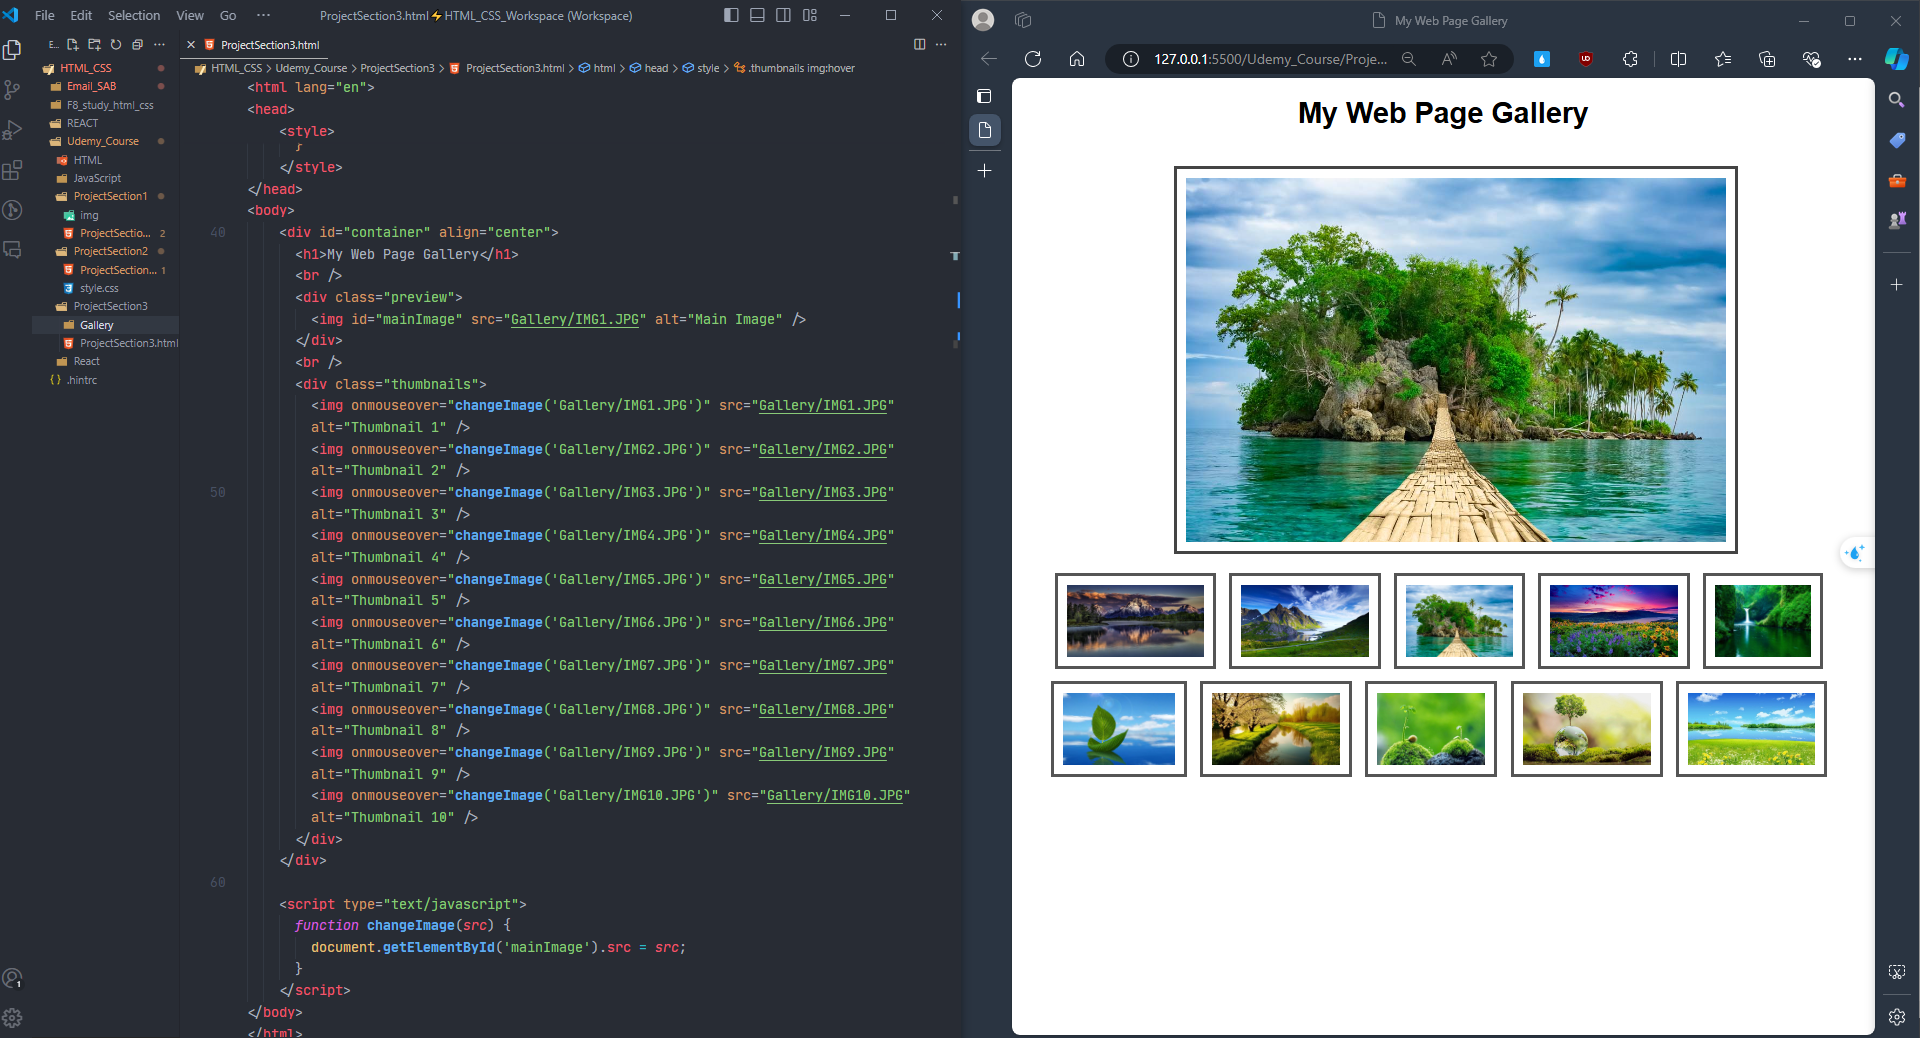
\includegraphics[width=0.9\linewidth]{img/Capture10.PNG}
		      \caption{A simple gallery website by HTML, CSS, and JavaScript (The main image will enlarge if you hover over it)}
	      \end{figure}


	\item \textbf{Content 4: React.} I am introduced to React, a popular JavaScript library for building user interfaces. I learn how to create components, manage state, and handle events in React applications. This is a simple calculator application built with React. It can perform basic arithmetic operations like addition, subtraction, multiplication, and division. It also has a clear button to clear the input field. Because this is the first project I've done, so inevitably copy existing source code to learn and understand how it works. I will try to understand the code and make some changes to it.
	      \begin{figure}[H]
		      \centering
		      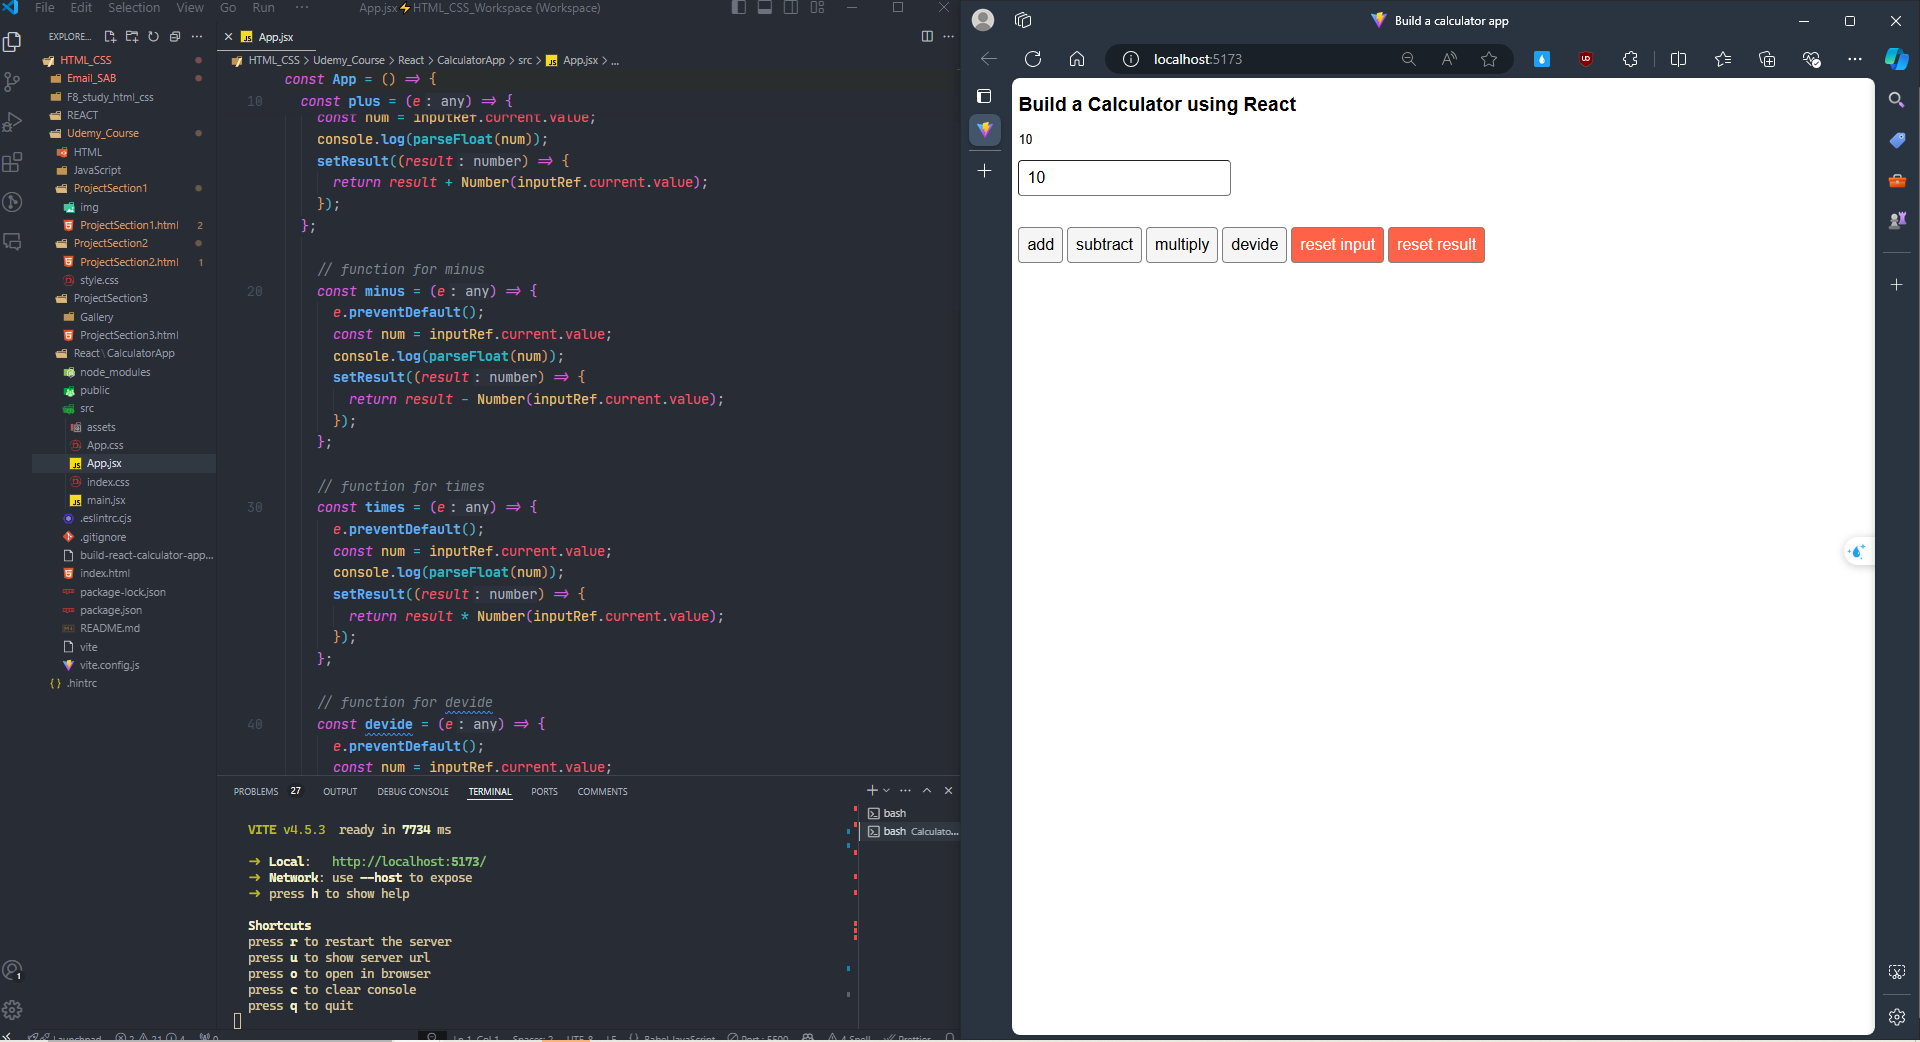
\includegraphics[width=1\linewidth]{img/Capture11.PNG}
		      \caption{A simple calculator app by React}
	      \end{figure}
\end{itemize}
\pagebreak
\section{Đánh giá}
\subsection{Bảng tự đánh giá các yêu cầu đã hoàn thành}

\begin{center}
\begin{table}[H]
    \centering
    \caption{Bảng tự đánh giá bài 1}
    \renewcommand{\arraystretch}{1.4}
    \begin{tabular}{|l|p{\dimexpr0.6\linewidth-2\tabcolsep}|c|}
    \hline
    \textbf{STT} & \textbf{Yêu cầu}            & \textbf{Mức độ hoàn thành} \\ \hline
    1            &  Nhập vào số nguyên X (4 byte) có dấu hãy "đọc" dãy bit nhị phân của X và xuất ra màn hình.       & 100\%          \\ \hline
    2            & Cho mảng 1 chiều A gồm 32 phần tử là các số 0 hoặc 1. Hãy xây dựng số nguyên X 4 byte có các bit giống với các phần tử mảng A, sau đó xuất X ra màn hình.
    & 100\%          \\ \hline
                & \textbf{Tổng cộng}               &\textbf{100\%}           \\ \hline
    \end{tabular}
    \label{tab:mytable}
\end{table}

  \begin{table}[H]
        \centering
        \caption{Bảng tự đánh giá bài 2}
        \renewcommand{\arraystretch}{1.4}
        \begin{tabular}{|l|p{\dimexpr0.6\linewidth-2\tabcolsep}|c|}
        \hline
        \textbf{STT} & \textbf{Yêu cầu}            & \textbf{Mức độ hoàn thành} \\ \hline
        1            &  Thực hiện phép tính cộng   & 100\%          \\ \hline
        2            &  Thực hiện phép tính trừ      & 100\%          \\ \hline
        3            &  Thực hiện phép tính nhân theo thuật toán Booth      & 100\%          \\ \hline
        4            &  Thực hiện phép tính chia lấy phần nguyên      & 100\%          \\ \hline
        5            &  Thực hiện phép tính chia lấy phần dư      & 100\%          \\ \hline
                    & \textbf{Tổng cộng}               &\textbf{100\%}           \\ \hline
      \end{tabular}
        \label{tab:mytable2}
  \end{table}
\end{center}

\subsection{Đánh giá tổng thể mức độ hoàn thành của bài nộp}

Bài nộp đã hoàn thành đầy đủ các yêu cầu đề ra trong bài tập. Tất cả các yêu cầu đều đã được cài đặt và kiểm thử thành công. Tổng thể, bài nộp đã hoàn thành 100\% các yêu cầu đề ra.

\end{document}